\documentclass[10pt, twocolumn]{article}
\usepackage[margin=1in]{geometry}                % See geometry.pdf to learn the layout options. There are lots.
\geometry{letterpaper}                   % ... or a4paper or a5paper or ... 
%\geometry{landscape}                % Activate for for rotated page geometry
%\usepackage[parfill]{parskip}    % Activate to begin paragraphs with an empty line rather than an indent
\usepackage{graphicx}
\usepackage{amssymb}
\usepackage{epstopdf}
\usepackage{subfigure}
\DeclareGraphicsRule{.tif}{png}{.png}{`convert #1 `dirname #1`/`basename #1 .tif`.png}

\title{Analyzing Encrypted Web Traffic with Single- and Multi-Class SVMs}
\author{Emily Stark}
\date{\today}                                          % Activate to display a given date or no date

\begin{document}
\maketitle
%\section{}
%\subsection{}

\section{Introduction}
Web users, especially those in regions with censored 
Internet access, often use encryption in conjunction 
with anonymizing proxies to conceal which website 
they are visiting. For example, a user whose government 
restricts access to \texttt{https://www.facebook.com} can choose a 
proxy in an uncensored region, and use that proxy to 
forward encrypted HTTP requests and responses to and 
from Facebook. In theory, the censoring entity cannot determine from 
the user's encrypted traffic that the user is visiting 
Facebook. However, encryption does not conceal the direction, 
size, and timing of the packets that a user's web browsing 
generates. In practice, this small amount of information can 
be enough to determine the website that the user is visiting.

This problem is naturally phrased as a supervised learning 
problem. Given a set of packet traces, where each trace is labelled 
with the website that a user visited to generate it, we would 
like to determine the website that a user visited to generate a new, 
unlabeled trace. The point of training such a classifier is not 
necessarily to make it easier for a censor to do its job, but rather 
to understand the security guarantees that a user gets from using 
an anonymizing proxy to forward encrypted web traffic, as well as 
the effectiveness of proposed defenses against traffic analysis. 
One such proposed defense is to generate a background request to a 
random website for every encrypted request to a sensitive website~\cite{torfingerprinting}. 
This defense, which I will refer to as the random-visit defense, 
attempts to confuse the classifier by the addition of random 
noise to the traffic generated by a visit to a sensitive website.

In this project, I applied support vector machine (SVM) classifiers 
to the problem of determining the source website of a stream of 
encrypted web traffic. My goals were 1.) to train a SVM to 
effectively classify traces of encrypted packets into their source 
websites, and 2.) to show that SVMs can be used to break the random-visit 
defense described above. While SVMs have been used before for 
encrypted traffic analysis~\cite{SOMETHING}, the random-visit defense 
is a very recent proposal and has not been well-studied yet.

Previous work classifies encrypted traffic analysis into two settings: 
closed world and open world. In the closed world setting, we assume that 
the user visits one of a small number of websites over an encrypted, 
anonymized connection, and the censor wishes to determine which website 
the user is visiting. In the open world problem, which is much harder, the 
censor has a small list of offensive websites that it wishes to block, but 
the user might visit any website on the Internet. The censor wishes to 
recognize when the user is visiting one of the offensive websites, and which 
of the offensive websites is being visited. I used SVM-based techniques to 
perform traffic analysis in both a very small closed-world setting and an 
open-world setting.

Below I summarize the tasks that I completed for this project.
\begin{itemize}
\item \textbf{Data generation and preprocessing.} I generated packet 
traces of visits to HTTPS websites, both with and without random 
background visits. From these traces, I generated a feature vector for 
each visit. This process is described in more detail in Section~\ref{sec:data}. 
\item \textbf{Training binary and multiclass SVMs.} I used the 
generated data to train several types of SVMs from the Python scikits-learn 
library~\cite{sklearn}. These included a binary SVM, as well as one-vs-all
and one-vs-one multiclass SVMs based on a binary SVM. I implemented $k$-fold cross-validation 
to determine the SVM parameters.
\item \textbf{Implementing a multiclass SVM and a single-class SVM for anomaly detection.} 
I built a multiclass SVM using the Python \texttt{cvxopt} library~\cite{cvxopt}.
 To investigate the 
open-world setting, I also built and trained a single-class SVM to perform 
anomaly detection.
\item \textbf{Designing and implementing a custom dimensionality reduction algorithm.} 
Because \texttt{cvxopt} does not scale to very large problems, the feature vectors from the 
packet traces were too large to run on the multiclass and single-class SVMs that I built. 
I designed a feature selection algorithm that uses data from website visits without the 
random-visit defense to select features for the data generated using the random-visit defense.
\end{itemize}

All the code that I wrote for this project is available online~\cite{github}.

\section{Related work}

Much previous work has analyzed encrypted traffic to reveal the destination website or 
even uncover sensitive information entered by the user on a HTTPS website. Early
approaches simply fingerprinted websites by recording the sizes of objects generated 
by a visit to the website~\cite{safeweb}. Since then, various machine learning 
and data mining techniques, such as Jaccard coefficients and multinomial naive Bayes classifiers,
have been applied to the encrypted traffic analysis problem~\cite{herrmann,liberatore}. 
A recent work showed that SVMs are an effective traffic analysis technique~\cite{tor}, even 
against protocols such as Tor (an anonymity network) that employ pipelining, which makes 
traffic analysis more difficult. This work proposed the random-visit defense discussed above. In 
this project I investigated the effectiveness of the random-visit defense in analyzing 
SSL-encrypted web traffic.

\section{Data generation and preprocessing}

In this paper, I will refer to a \textit{target site} as one of the HTTPS websites that a censoring 
entity wants to block, and that a user tries to visit via an anonymizing proxy.
 The target site is the label in the classification 
problem. The \textit{background site} is the random website loaded in the background when a 
user is using the random-visit defense.

I generated two data sets for this project. The \textit{single-visit} data set consists of packet 
traces from individual visits to a small set of target sites. The \textit{multi-visit} data set 
consists of packet traces from individual visits to a small set of target sites, where each visit 
happened concurrently with a visit to a random background site.

I used 8 popular HTTPS websites (two banks, two file sharing applications, two social networks, 
Google, and the Tor website) as target sites. The list of websites is located in \texttt{gen\_data.py}.
In future, this work could be made much more convincing by increasing the number of target sites 
to several hundred, but for this project I limited the closed-world setting to a few websites 
because of limited computational resources. (I ran all experiments on my Macbook Pro laptop, and 
for some classifiers, even with the small list of target sites, I had to limit the amount of data 
used in training in order to not run out of memory. I discuss this limitation in greater detail 
in Section~\ref{sec:multiclassimplementation}.)

The background sites were chosen randomly from a list of 5000 of the most popular websites~\cite{alexa}. 
While the background sites were visited over HTTP, I only used information such as packet timings and 
lengths that would be available if HTTPS background sites were used. A real deployment of the 
random-visit defense would use HTTPS-enabled sites as background sites; I only used HTTP sites as 
background sites in this project because a large list of HTTPS websites was not readily available.

\subsection{Data generation}

For the single-visit data set, I wrote a Python script (\texttt{gen\_data.py}) to visit each site 
in the list of target sites 30 times and record a packet trace with \texttt{tcpdump}. Each visit 
occurred in a new instance of Google Chrome (in incognito mode, to prevent the browser from 
using cached resources in subsequent visits).

For the multi-visit data set, I modified \texttt{gen\_data.py} to, on each target site visit, 
simultaneously open a second tab and load a randomly selected background site in that tab. For the 
multi-visit data set, I recorded 60 visits to each target site instead of 30, since the multi-visit 
data set presents a harder classification problem and therefore having more training data is helpful.

\subsection{Preprocessing packet traces into feature vectors}
\label{sec:preprocessing}

\texttt{preprocess.py} uses \texttt{tcpdump} to parse the raw packet traces, and then translates 
each target site visit into a feature vector. I defined three features for each recorded packet: the 
time relative to the time of the first packet in the trace, the direction of the packet (to or from 
the user's machine), and the length of the packet. I padded each vector with $-1$ values so that all 
feature vectors in each data set were the same length. This selection of features led to large vectors 
with several thousand features. For the classifiers that were unable to handle such large feature vectors 
(my implementations of a multiclass SVM and a single-class SVM for anomaly detection, both using 
\texttt{cvxopt}), I designed and implemented a dimensionality reduction algorithm that I describe in 
Section~\ref{sec:dimred}.

\section{SVMs in the closed world setting}

For the closed world setting, I compared three multiclass SVMs:
\begin{itemize}
\item a one-vs-one multiclass SVM implemented in the scikits-learn library,
\item a one-vs-all multiclass SVM implemented in the scikits-learn library,
\item a multiclass SVM that I implemented using \texttt{cvxopt} (the implementation is 
described in Section~\ref{sec:multiclassimplementation}).
\end{itemize}

I investigated the performance of these SVMs on both the single-visit and multi-visit data. 
The training data was a list of feature vectors, where each feature vector corresponds to a 
packet trace from a visit to a target site, as described in Section~\ref{sec:preprocessing}.

I implemented $k-$fold cross-validation for each SVM to choose parameters. I also used 
cross-validation to observe how the classifier's performance improves with the addition of more data 
and how it suffers when more classes are introduced. Data from the cross-validation process is shown 
in Section~\ref{sec:crossvalidation}.

\subsection{Multiclass SVM implementation}
\label{sec:multiclassimplementation}

\subsection{Cross-validation for parameter tuning}
\label{sec:crossvalidation}

\begin{figure*}
\begin{center}
\subfigure[Single-visit data with full dimensionality.]{
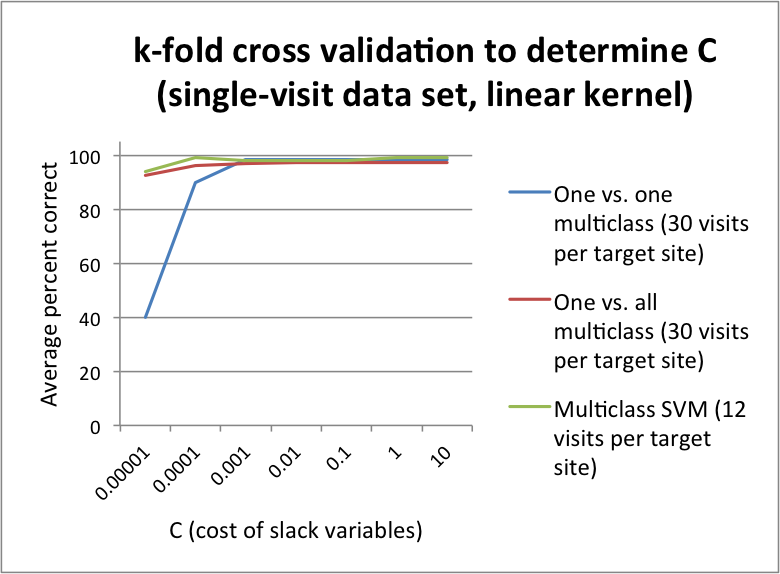
\includegraphics[scale=0.6]{graphs/single_visit_c.png}
\label{fig:kfoldc-single}
}
\subfigure[Multi-visit data with dimensionality reduced to 50 features.]{
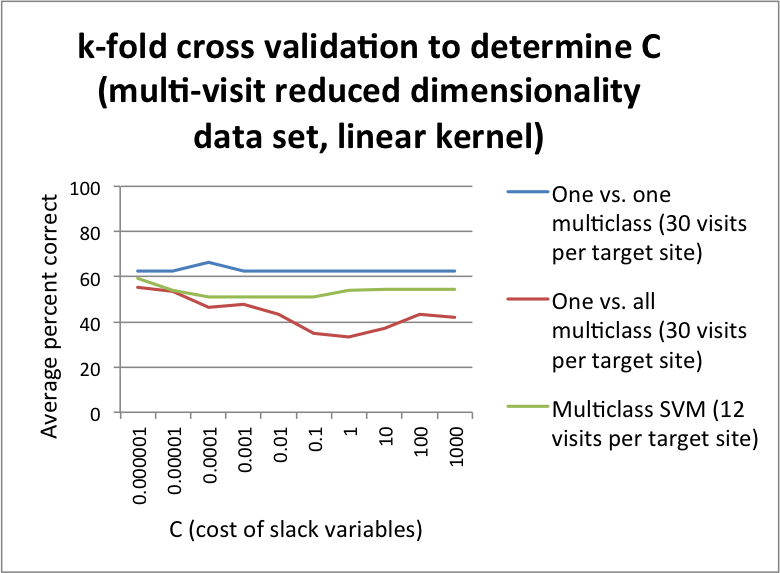
\includegraphics[scale=0.6]{graphs/multi_visit_c.png}
\label{fig:kfoldc-multi}
}
\caption{$k$-fold cross-validation results (with $k=6$) for tuning $c$, the cost associated with 
each slack variable. The smaller size of the training data for the multiclass SVM is due to 
limited computational resources.}
\label{fig:kfoldc}
\end{center}
\end{figure*}


\subsection{Performance results and analysis}

\textbf{TODO: insert perf results}

I briefly explored using the radial basis function as a kernel in the one-versus-one multiclass 
SVM, but I could not find parameters that outperformed the linear kernel. For example, using $k$-fold 
cross-validation with $k=6$ and the multi-visit data with 30 visits per target site, the best choice of 
parameters that I was able to find for the linear and RBF kernels led to average performance of about 
$30\%$ correct for both kernels. Assuming that I didn't miss some better choice of parameters for the 
RBF kernel, this result suggests that the data is mostly linearly separable with outliers: the RBF kernel 
does no better than the linear kernel, and it can do worse by overfitting.

\section{A single-class SVM for the open world setting}

For the open world setting, I implemented a single-class SVM with kernels, using the 
\texttt{cvxopt} library.

\subsection{Single-class SVM implementation}

\subsection{Cross-validation for parameter tuning}

\subsection{Performance results and analysis}

\section{Dimensionality reduction}
\label{sec:dimred}

Table~\ref{tab:dimred-kfold} shows a SVM's performance as the number of features varies. The dimensionality 
reduction algorithm definitively increases performance over the original feature vectors, and performance 
seems to improve as the number of features gets smaller. This suggests that there are a small number of 
packets that distinguish each target website, and the dimensionality reduction algorithm is effective at 
extracting these features while removing noise.

\begin{table}
\caption{$k$-fold cross-validation performance of a one-vs-one multiclass SVM as the dimensionality of 
the data is varied. $c$ is fixed at $1.0$ and $k$ is fixed at $6$. The data is the multi-visit data set 
with 30 visits to each target site.}
\begin{center}
\begin{tabular}{|r|r|}
\hline
Number of features & Average percent correct \\
\hline
30 & 69\% \\
\hline
50 & 61\% \\
\hline
70 & 59\% \\
\hline
90 & 60\% \\
\hline
110 & 59\% \\
\hline
All original features & 36\% \\ \hline
\end{tabular}
\end{center}
\label{tab:dimred-kfold}
\end{table}%


\end{document}  